\section{Correlations}
\label{sec:correlations}

\noindent The correlation coefficient is a measure of the linear dependence between two variables and is calculated as follows:

\begin{equation}
r = \frac{\sum_{i=1}^{n}(X_i - \bar{X})(Y_i - \bar{Y})}{\sqrt{\sum_{i=1}^{n}(X_i - \bar{X})^2}\sqrt{\sum_{i=1}^{n}(Y_i - \bar{Y})^2}}
\end{equation}

\noindent where $r$ is the correlation coefficient and has a value between +1 and -1.

\noindent If $r$ = +1 it corresponds to a positive perfect correlation as $X$ increases so does $Y$. Similary if $r$ = -1 it corresponds to a negative perfect correlation, as $X$ increases $Y$ decreases. A correlation coefficient of 0 means that there is no correlation between the two variables. \cite{corrcoeff}.


\subsection{Distances Travelled}
\label{sec:corelldistance}

Using an outlier that has previously been found, in this case Elsa Orilla, the distance data from such outlier can be compared for each day in order to have another form of analysis to confirm that it is an anomaly. \\

\begin{figure}[H]
\centering
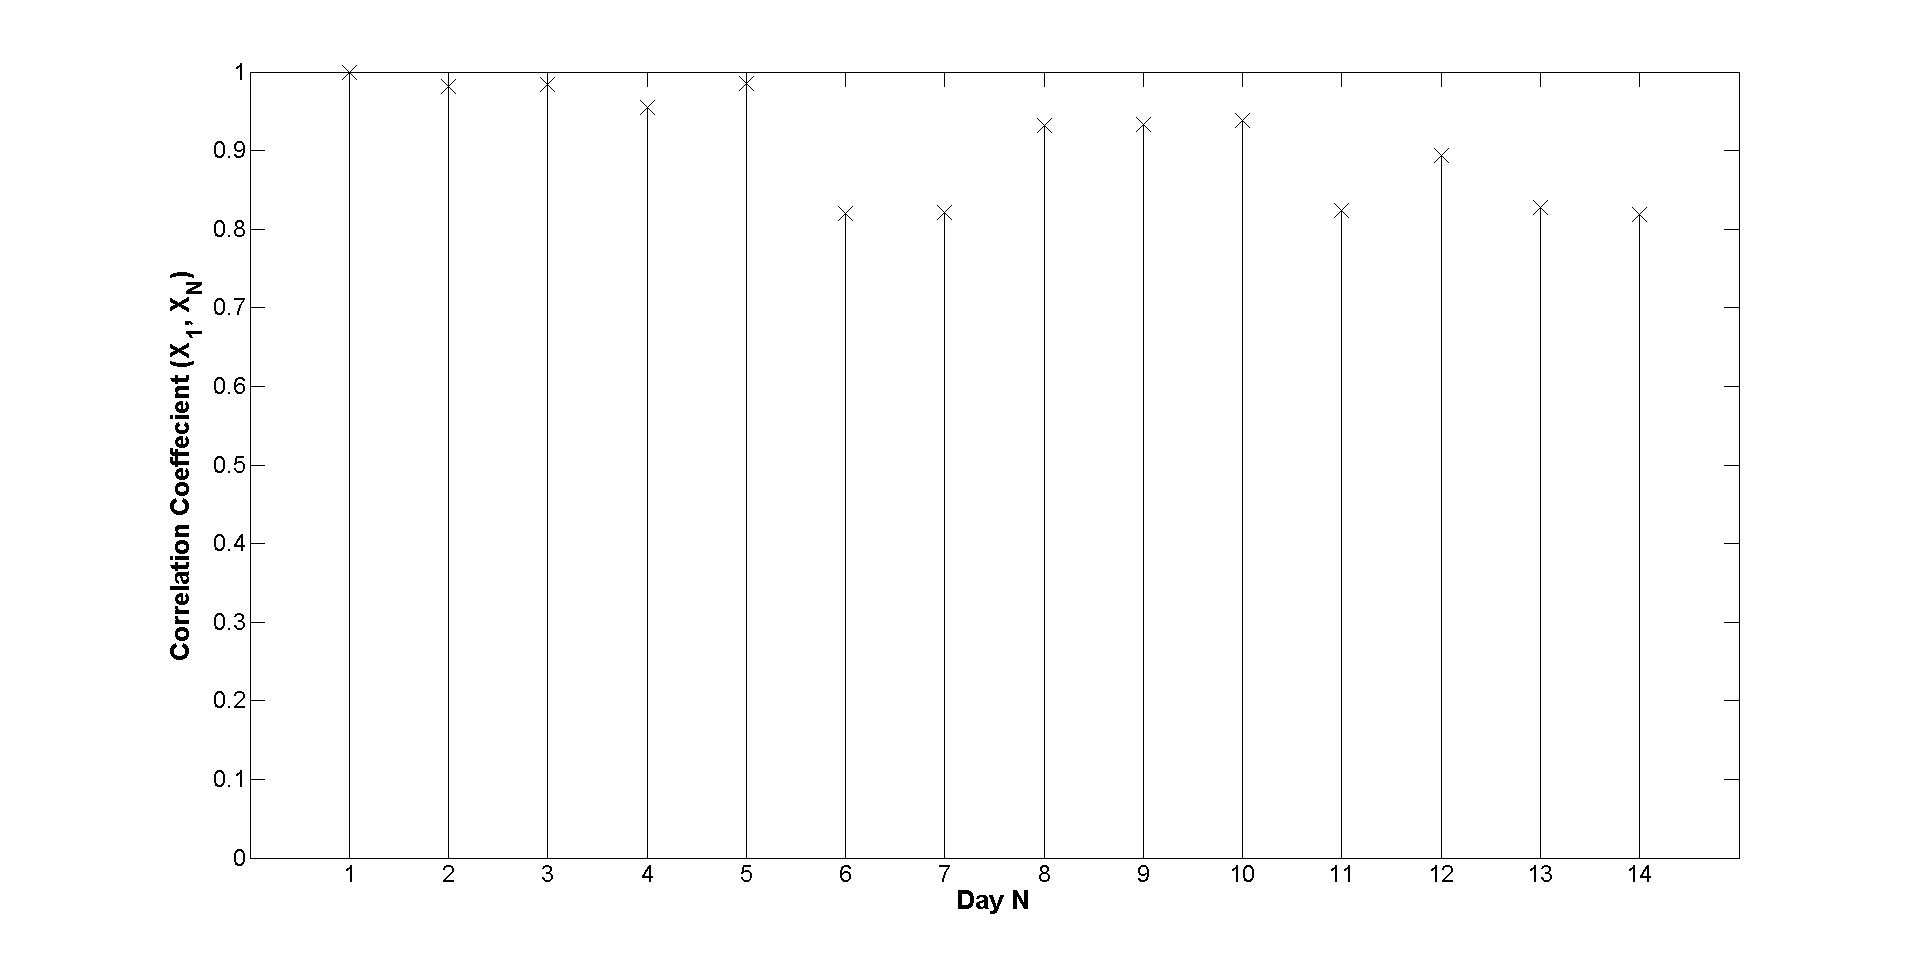
\includegraphics[width=1.0\textwidth]{CorrelateDistanceID28.png}
\caption{\label{fig:CorrelateDistanceID28} The correlation coefficients, for distance travelled by Elsa Orilla, between day 1 and day 14.}
\end{figure}

\noindent Figure \ref{fig:CorrelateDistanceID28} shows this correlation. The distance data is correlated in such a way that each day is compared to the first day in the time period. From Figure \ref{fig:CorrelateDistanceID28}  it can be seen that each day has a fairly high correlation coefficient, however this is to be expected because the distance will always be increasing as it is the cumulitive distance. Nonetheless there are some values that are significantly lower than others and this shows that on the day where such a value appears, the distances travelled were different to those travelled on day 1. \\ 
